\documentclass [aspectratio=169]{beamer}
\beamertemplatenavigationsymbolsempty
\usetheme{Boadilla}
\usepackage{textpos} % package for the positioning
\usepackage[]{graphicx}
\usepackage{graphicx}
\usepackage{float}
\usepackage{hyperref}
\usepackage{caption}
\usepackage{subcaption}
\usepackage{algorithm,algpseudocode}
\usepackage[export]{adjustbox}
\usepackage{tikz}
\usepackage[square,numbers]{natbib}
\usepackage[byname]{smartref}
\usetikzlibrary{positioning}
\usetikzlibrary{arrows, shapes, decorations, automata, backgrounds, fit, petri, calc}

\newcommand*{\logofont}{\fontfamily{phv}\selectfont}

\definecolor{uwopurple}{RGB}{79,38,131} % official purple color for uwo

\title[]{\vspace{60pt} \\
The \bbonu\ Lonely Hearts Club Band} % Change the lecture topic right here!
%\subtitle{n}
\author[]{J.J. Gómez Cadenas}
\institute[]{Donostia International Physics Center}
\date{\today}

% Math notations
\newtheorem{thm}{Theorem}[section]
\newtheorem{lem}[thm]{Lemma}

\newtheorem{defn}[thm]{Definition}
\newtheorem{eg}[thm]{Example}
\newtheorem{ex}[thm]{Exercise}
\newtheorem{conj}[thm]{Conjecture}
\newtheorem{cor}[thm]{Corollary}
\newtheorem{claim}[thm]{Claim}
\newtheorem{rmk}[thm]{Remark}

\newcommand{\ie}{\emph{i.e.} }
\newcommand{\cf}{\emph{cf.} }
\newcommand{\into}{\hookrightarrow}
\newcommand{\dirac}{\slashed{\partial}}
\newcommand{\bbonu}{\ensuremath{\beta\beta0\nu}}
\newcommand{\bbtnu}{\ensuremath{\beta\beta2\nu}}
\newcommand{\mbb}{\ensuremath{m_{\beta\beta}}}
\newcommand{\qbb}{\ensuremath{Q_{\beta\beta}}}
\newcommand{\mbbsq}{\ensuremath{m_{\beta\beta}^2}}
\newcommand{\tonu}{\ensuremath{(T_{1/2}^{0\nu})^{-1}}}
\newcommand{\gonu}{\ensuremath{G^{0\nu}}}
\newcommand{\monu}{\ensuremath{|M^{0\nu}|^2}}
\newcommand{\XE}{\ensuremath{{}^{136}{\rm Xe}}}
\newcommand{\GE}{\ensuremath{{}^{76}{\rm Ge}}}
\newcommand{\TE}{\ensuremath{{}^{130}{\rm Te}}}
\newcommand{\MO}{\ensuremath{{}^{100}{\rm Mo}}}
\newcommand{\R}{\mathbb{R}}
\newcommand{\C}{\mathbb{C}}
\newcommand{\Z}{\mathbb{Z}}
\newcommand{\N}{\mathbb{N}}
\newcommand{\Q}{\mathbb{Q}}
\newcommand{\LieT}{\mathfrak{t}}
\newcommand{\T}{\mathbb{T}}
\newcommand{\A}{\mathds{A}}
\newcommand{\E}{\mathbb{E}}
\newcommand{\Prob}{\mathbb{P}}
\newcommand{\Var}{\text{Var}}
\newcommand\equalhat{%
\let\savearraystretch\arraystretch
\renewcommand\arraystretch{0.3}
\begin{array}{c}
\stretchto{
    \scalerel*[\widthof{=}]{\wedge}
    {\rule{1ex}{3ex}}%
}{0.5ex}\\ 
=%
\end{array}
\let\arraystretch\savearraystretch
}

% set color
\setbeamercolor{title in head/foot}{bg=white}
\setbeamercolor{author in head/foot}{bg=white}
\setbeamercolor{date in head/foot}{fg=uwopurple}
\setbeamercolor{date in head/foot}{bg=white}
\setbeamercolor{title}{fg=uwopurple}
\setbeamerfont{title}{series=\bfseries}
\setbeamercolor{frametitle}{fg=uwopurple}
\setbeamerfont{frametitle}{series=\bfseries}
\setbeamercolor{block title}{bg=uwopurple!30,fg=black}
\setbeamercolor{item}{fg=uwopurple}
\setbeamercolor{caption name}{fg=uwopurple!70!}


% set logo at non-title pages
%\logo{\includegraphics[height=0.9cm]{dipc.png}\vspace*{-.45\paperheight}\hspace*{.50\paperwidth}}

\begin{document}

{
\setbeamertemplate{logo}{}
\begin{frame}
    \titlepage
    \begin{textblock*}{4cm}(0.5cm,-7.3cm)
        \includegraphics[width=4cm]{dipc.png}
    \end{textblock*}
    \begin{textblock*}{8cm}(5.0cm,-7.0cm)
        \huge \color{uwopurple}{$\Bigr\rvert$ \hspace{0.15cm} \textbf{Lecture 1}} % Change the lecture # right here! 
    \end{textblock*}
\end{frame}
}

\begin{frame}{Majorana Neutrinos in one slide}
%\begin{columns}
%\column{0.40\textwidth}
 \begin{textblock*}{4cm}(1.7cm,-2.7cm)
\includegraphics[scale=0.30]{majorananu.png}
 \end{textblock*}

% \column{0.5\textwidth}
%The neutrino is made, like in the Escher’s tableau of black and white chevaliers.   
%\end{columns}
\end{frame}

%%%

\begin{frame}{Majorana neutrinos \& a recipe for the Universe}
\includegraphics[scale=0.40]{Universe.png}
\end{frame}

%%

\begin{frame}{Majorana neutrinos are double agents}

\includegraphics[scale=0.112]{doubleAgent.png}
\end{frame}


\begin{frame}{Are neutrinos Majorana Particles?}

\begin{columns}
\column{0.50\textwidth}
\includegraphics[scale=0.35]{DoubleOrNothing.png}

 \column{0.50\textwidth}
To find out play this game!   
\end{columns}
\end{frame}

%%%

\begin{frame}{$\beta\beta2\nu$. An oddity of Nature}

\begin{columns}
\column{0.5\textwidth}
\includegraphics[scale=0.40]{xebb2nu.png}
\includegraphics[scale=0.40]{betabetaisotopes.png}


 \column{0.50\textwidth}
$\bullet~$ Double beta decay is a rare nuclear transition in which a nucleus with Z protons decays into a nucleus with Z + 2 protons and the same mass number A. The decay can occur only if the initial nucleus is less bound than the final nucleus, and both more than the intermediate one.

$\bullet~$ Such a condition is fulfilled by 35 nuclides in nature because of the nuclear pairing force ensuring that nuclei with even Z and N are more bound than the odd-odd nuclei with the same A = Z + N.

$\bullet~$ Being a second-order process in $G_F$, the lifetime of $\beta\beta2\nu$ processes is very long ($\sim 10^{20}$~y in Xe).
 
\end{columns}
\end{frame}

\begin{frame}{$\beta\beta0\nu$. If and only if neutrinos are Majorana Particles}

\begin{columns}
\column{0.50\textwidth}
\includegraphics[scale=0.25]{bb0nu.png}

 \column{0.50\textwidth}
$\bullet~$ Inverse of the lifetime is proportional to $m_{\beta\beta}^2$. For small neutrino masses this results in very long lifetimes (effect vanishes if the neutrino mass is zero). 

$\bullet~$ No neutrinos are emitted in the process, leading to a ``golden signature''.

$\bullet~$ Knowledge of NME necessary (and difficult).
 
\end{columns}
\end{frame}

%%%
\begin{frame}{Exercise 1}

$\bullet~$ Give a qualitative argument (using neutrino helicity) to argue that the amplitude of  $\beta\beta0\nu$ must be proportional to m$_{\beta\beta}$, and thus lifetime proportional to m$_{\beta\beta}^2$.
\end{frame}

%%%

\begin{frame}{Nuclear Matrix Elements and Phase Space}
\begin{figure}
\includegraphics[scale=0.20]{nme2.png}
\caption{1. NME and Phase Space for several isotopes}

\end{figure}
\end{frame}

%%%

%%%
\begin{frame}{Exercise 2}

$\bullet~$ Suppose that you have established a limit for the lifetime of a given \bbonu\ isotope, 
\tonu. To obtain the sensitivity to the physical parameter \mbbsq, one can simply write:
\[
\mbbsq = \frac{\tonu}{\gonu\cdot\monu}
\]

From the data in figure 1, use QRPA (red bars) to estimate the central value and the error of \gonu\ and \monu\ for \GE\, \TE\ and \XE\ and \MO\. Then obtain the uncertainty in \mbb\ for 
$\tonu \sim 10^{27}$~y and $\tonu \sim 10^{28}$~y. Which range of \mbb\ do you obtain? What do you conclude?

\end{frame}

%%%%%

\begin{frame}{Lonely Harts sorrows (1)}
\begin{columns}
\column{0.50\textwidth}
\includegraphics[scale=0.35]{lonelyhearts.png}

 \column{0.50\textwidth}
$\bullet~$ ¿Have you noticed? You need to improve one order of magnitude the sensitivity to \tonu\ to improve a mere factor 3 the sensitivity to \mbb\ (in the case of no background). Darn the square! Nothing you can do about this, though, is just Nature being nasty with you. 

$\bullet~$ ¿Have you noticed? NME uncertainty translates into a huge uncertainty in \mbb\ sensitivity (darn the square again!). Here we can improve, using better models as in figure. If you are curious on how to improve NME, see for example: \url{https://link.springer.com/article/10.1007/s40766-023-00049-2} and references therein.  

\end{columns}
\end{frame}

%%%

\begin{frame}{Majorana Landscape}

%\begin{columns}
%\column{0.40\textwidth}
\includegraphics[scale=0.25]{landscape2.png}
%\column{0.40\textwidth}

%\includegraphics[scale=0.40]{ordering2.png}


%$\bullet~$ When representing $m_{\beta\beta}$~as a function of the mass of the lightest neutrino $m_l$, one obtains two possible landscapes, one for the ``Normal Ordering'' (NO) and the other for the ``Inverse Ordering" (IO). 
%
%$\bullet~$ Color shows probability. 
%\end{columns}

\end{frame}
%%%

\begin{frame}{The challenge for $\beta\beta0\nu$ experiments}

\begin{columns}
\column{0.50\textwidth}
\includegraphics[scale=0.25]{landscapes.png}

 \column{0.50\textwidth}
$\bullet~$ Uncertainties in NME (exercise 2) translate in variations of almost one order of magnitude in expected lifetime (and thus expected rate) for a given $m_{\beta\beta}$. 

$\bullet~$ Current generation of experiments have reached $4 \times 10^{26}$~y (KamLAND-Zen), which barely scrapes the IO, even in the most optimistic case. 

$\bullet~$ Next generation of experiments target a sensitivity of $\sim 10^{27}$~y, which would cover IO only in the optimistic scenarios. 

$\bullet~$ Next-to-next generation of experiments target a sensitivity of $\sim 10^{28}$~y, which would cover a fraction of the NO only in the optimistic scenarios. 
\end{columns}
\end{frame}

%%%%

\begin{frame}{How difficult is to reach $T_{\beta\beta0\nu} \sim 10^{27} (~10^{28})$~y?}

\begin{columns}
\column{0.50\textwidth}
\includegraphics[scale=0.23]{strawdet.png}
\includegraphics[scale=0.30]{pajar.png}

 \column{0.50\textwidth}
$\bullet~$ Requires to build detectors(s) deploying enough mass (e.g., enough nuclei of the chosen isotope to play the ``lottery of the impossible") and exploiting the distinctive signature(s) of the $\beta\beta0\nu$ decay. 

$\bullet~$ Requires to suppress the natural radioactivity backgrounds, as well as the impact of cosmic rays (thus, underground laboratories such as LNGS, LSC, SNOLAB, etc. are a must)

\end{columns}
\end{frame}

%%%%

\begin{frame}{An ideal ${\beta\beta0\nu}$ experiment (1)}

\begin{columns}
\column{0.50\textwidth}
\includegraphics[scale=0.43]{idealdet.png}


 \column{0.50\textwidth}
$\bullet~$ Get yourself a detector with {\em perfect energy resolution}. 

$\bullet~$ Measure the energy of the emitted electrons and select those with 
$(T_1+T_2)/Q_{bb} = 1$.

$\bullet~$ Do not worry about backgrounds, a detector with perfect energy resolution suppresses them all. 

$\bullet~$ Count the number of observed events (they are all signal) and calculate the corresponding lifetime.

\end{columns}
\end{frame}

%%%%

\begin{frame}{An ideal ${\beta\beta0\nu}$ experiment (2)}

\begin{columns}
\column{0.50\textwidth}
\includegraphics[scale=0.70]{graxe.png}


 \column{0.50\textwidth}
$\bullet~$ Get yourself a detector with {\em perfect shielding}. 

$\bullet~$ Measure the energy of the emitted electrons and select those with 
$(T_1+T_2)/Q_{bb} \sim 1$.

$\bullet~$ Do not worry about external backgrounds, a detector with perfect shielding suppresses them all. 

$\bullet~$ But you need to worry about {\bf internal backgrounds}, e.g., \bbtnu\ and neutrino floor, as well as {\bf cosmogenic backgrounds}. If you combined perfect shielding with sufficiently good energy resolution, you also approach an ideal detector.  

\end{columns}
\end{frame}

%%%%

\begin{frame}{An ideal ${\beta\beta0\nu}$ experiment (3)}

\begin{columns}
\column{0.50\textwidth}
\includegraphics[scale=0.17]{idealtopo.png}


 \column{0.50\textwidth}
$\bullet~$ Get yourself a detector with {\em perfect signal signature}. 

$\bullet~$ Measure the energy of the emitted electrons and select those with 
$(T_1+T_2)/Q_{bb} \sim 1$.

$\bullet~$ Do not worry about external backgrounds, a detector with perfect signal signature suppresses them all. 

$\bullet~$ But you need to worry about  \bbtnu. If your energy resolution is not excellent, some of the intrinsic backgrounds will make it into your ROI. If you combined perfect signal signature with sufficiently good energy resolution, you approach an ideal detector. 

\end{columns}
\end{frame}

\begin{frame}{Perfect detectors do not exist}
\begin{columns}
\column{0.50\textwidth}

\includegraphics[scale=0.15]{nopefect.png}

 \column{0.50\textwidth}
$\bullet~$ Real detectors must somehow combine the best of the three ideal detectors discussed above. An energy resolution as good as possible, signal signatures as clear as possible  and as much shielding as possible.  

$\bullet~$ Of course, often enough one condition is, at least partially, add odds with the others.

 $\bullet~$ Last but not least you cannot choose freely your target material, it must be one of double-beta decaying isotopes. Some of those materials have physical and chemical properties that you can exploit for a detector, some don't, excluding them from the game. 

\end{columns}
\end{frame}
%%%%

\begin{frame}{Rates in the absence of backgrounds}
\begin{columns}
\column{0.50\textwidth}
\begin{figure}
\includegraphics[scale=0.43]{ratesbb0nu.png}
\caption{2. Rates in the absence of background}
\end{figure}

 \column{0.50\textwidth}
$\bullet~$ Rates depend on isotope (and on assumptions on NME). 

$\bullet~$ For Xenon (under the particular NME assumed in figure), one needs an exposure of 1 ton$\cdot$year to reach $m_{\beta\beta}$.

$\bullet~$ Caveat. Optimistic value of NME on plot.  

$\bullet~$ Differences between different isotopes is relevant, but differences between different models is larger. Experiments must use several isotopes to minimise uncertainty. 

\end{columns}
\end{frame}

%%%
\begin{frame}{Exercise 3}

$\bullet~$ Obtain the plot in figure 2, for \XE, \GE. \TE, and \MO. To do this, write
\[
N_{\bbonu} = \log{2} \frac{M_{\beta\beta} N_A}{W_{\beta\beta}}\cdot t \cdot \tonu
\]
Where M$_{\beta\beta}$ is the mass of isotope in your experiment, N$_A$ is Avogadro's number and
W$_{\beta\beta}$ the molar mass of the isotope. 

\begin{itemize}
\item  {\color{uwopurple} First obtain the sensitivity to \tonu as a function of $ M_{\beta\beta} \cdot t$. This can be done computing the value of \tonu\ that allows the observation of (exactly) one event for a given exposure.}
\item  {\color{uwopurple} Side question: is this a correct approach? If you don't like it propose a better method.}  
\item  {\color{uwopurple} Then, compute the values of \mbbsq\ corresponding to \tonu\ dividing by \gonu\ and \monu. Use QRPA, taking the central value of the red bars in figure. }
\item {\color{uwopurple} Finally, compute \mbb. How do you feel about taking the square root? 
%(you should feel bad, it will cost years of your life if you work in this business).
} 
\end{itemize}

\end{frame}

%%%



%%%%%

\begin{frame}{Backgrounds}
\begin{columns}
\column{0.40\textwidth}
\includegraphics[scale=0.43]{radiochains.png}

 \column{0.60\textwidth}
$\bullet~$ {\bf Intrinsic background, \bbtnu}.Can only be distinguished by measuring the energy of the emitted electrons, since the neutrinos escape the detector undetected. Good energy resolution is therefore essential to prevent the \bbtnu\ spectrum tail from spreading over the \bbonu\ ROI, or to cause pileup (in the case of isotopes with a fast \bbtnu\ mode such as \MO (CUPID).

$\bullet~$ Any process generating energy deposits in the detector active volume of the order of \qbb\ is a potential background in \bbonu\ searches. The background sources can be categorised as follows: {\bf radiogenic} (produced by natural radioactivity), {\bf cosmogenic} (produced by the action of cosmic rays) and {\bf heliogenic} (produced by the Sun). They can also be classified by whether they are internal or external to the detector.

\end{columns}
\end{frame}


\begin{frame}{Majorana's Beach}
%\begin{columns}
%\column{0.40\textwidth}
\includegraphics[scale=0.40]{beach.png}


 %\column{0.60\textwidth}
$\bullet~$ {\bf Lifetime of radiogenic backgrounds} is of the order of $10^{10}$~y. To explore \bbonu\ lifetimes of the order of $10^{27}$~y. Thus $S/N \sim 10^{17}$.

$\bullet~$ {\bf Majorana’s beach}: A beach with $10^{17}$~ grains of sand (70 km long and 1 km wide).

%\end{columns}
\end{frame}

\begin{frame}{Radiopurity}
\begin{columns}
\column{0.60\textwidth}
\includegraphics[scale=0.22]{radiospectrum.png}

Ambient background measured by a HPGe detector without and with (green) shield.

 \column{0.40\textwidth}
 
$\bullet~$ All \bbonu\  experiment must use materials with extremely low amounts of radioactive impurities. Selection, manufacturing, cleaning and installation of detector materials has to be conducted with extreme care in all \bbonu\  experiments, relying on radio-pure protocols at all times.

\end{columns}
\end{frame}

\begin{frame}{Anatomy of an ultra-low background Ge detector (LSC)}
%\begin{columns}
%\column{0.60\textwidth}
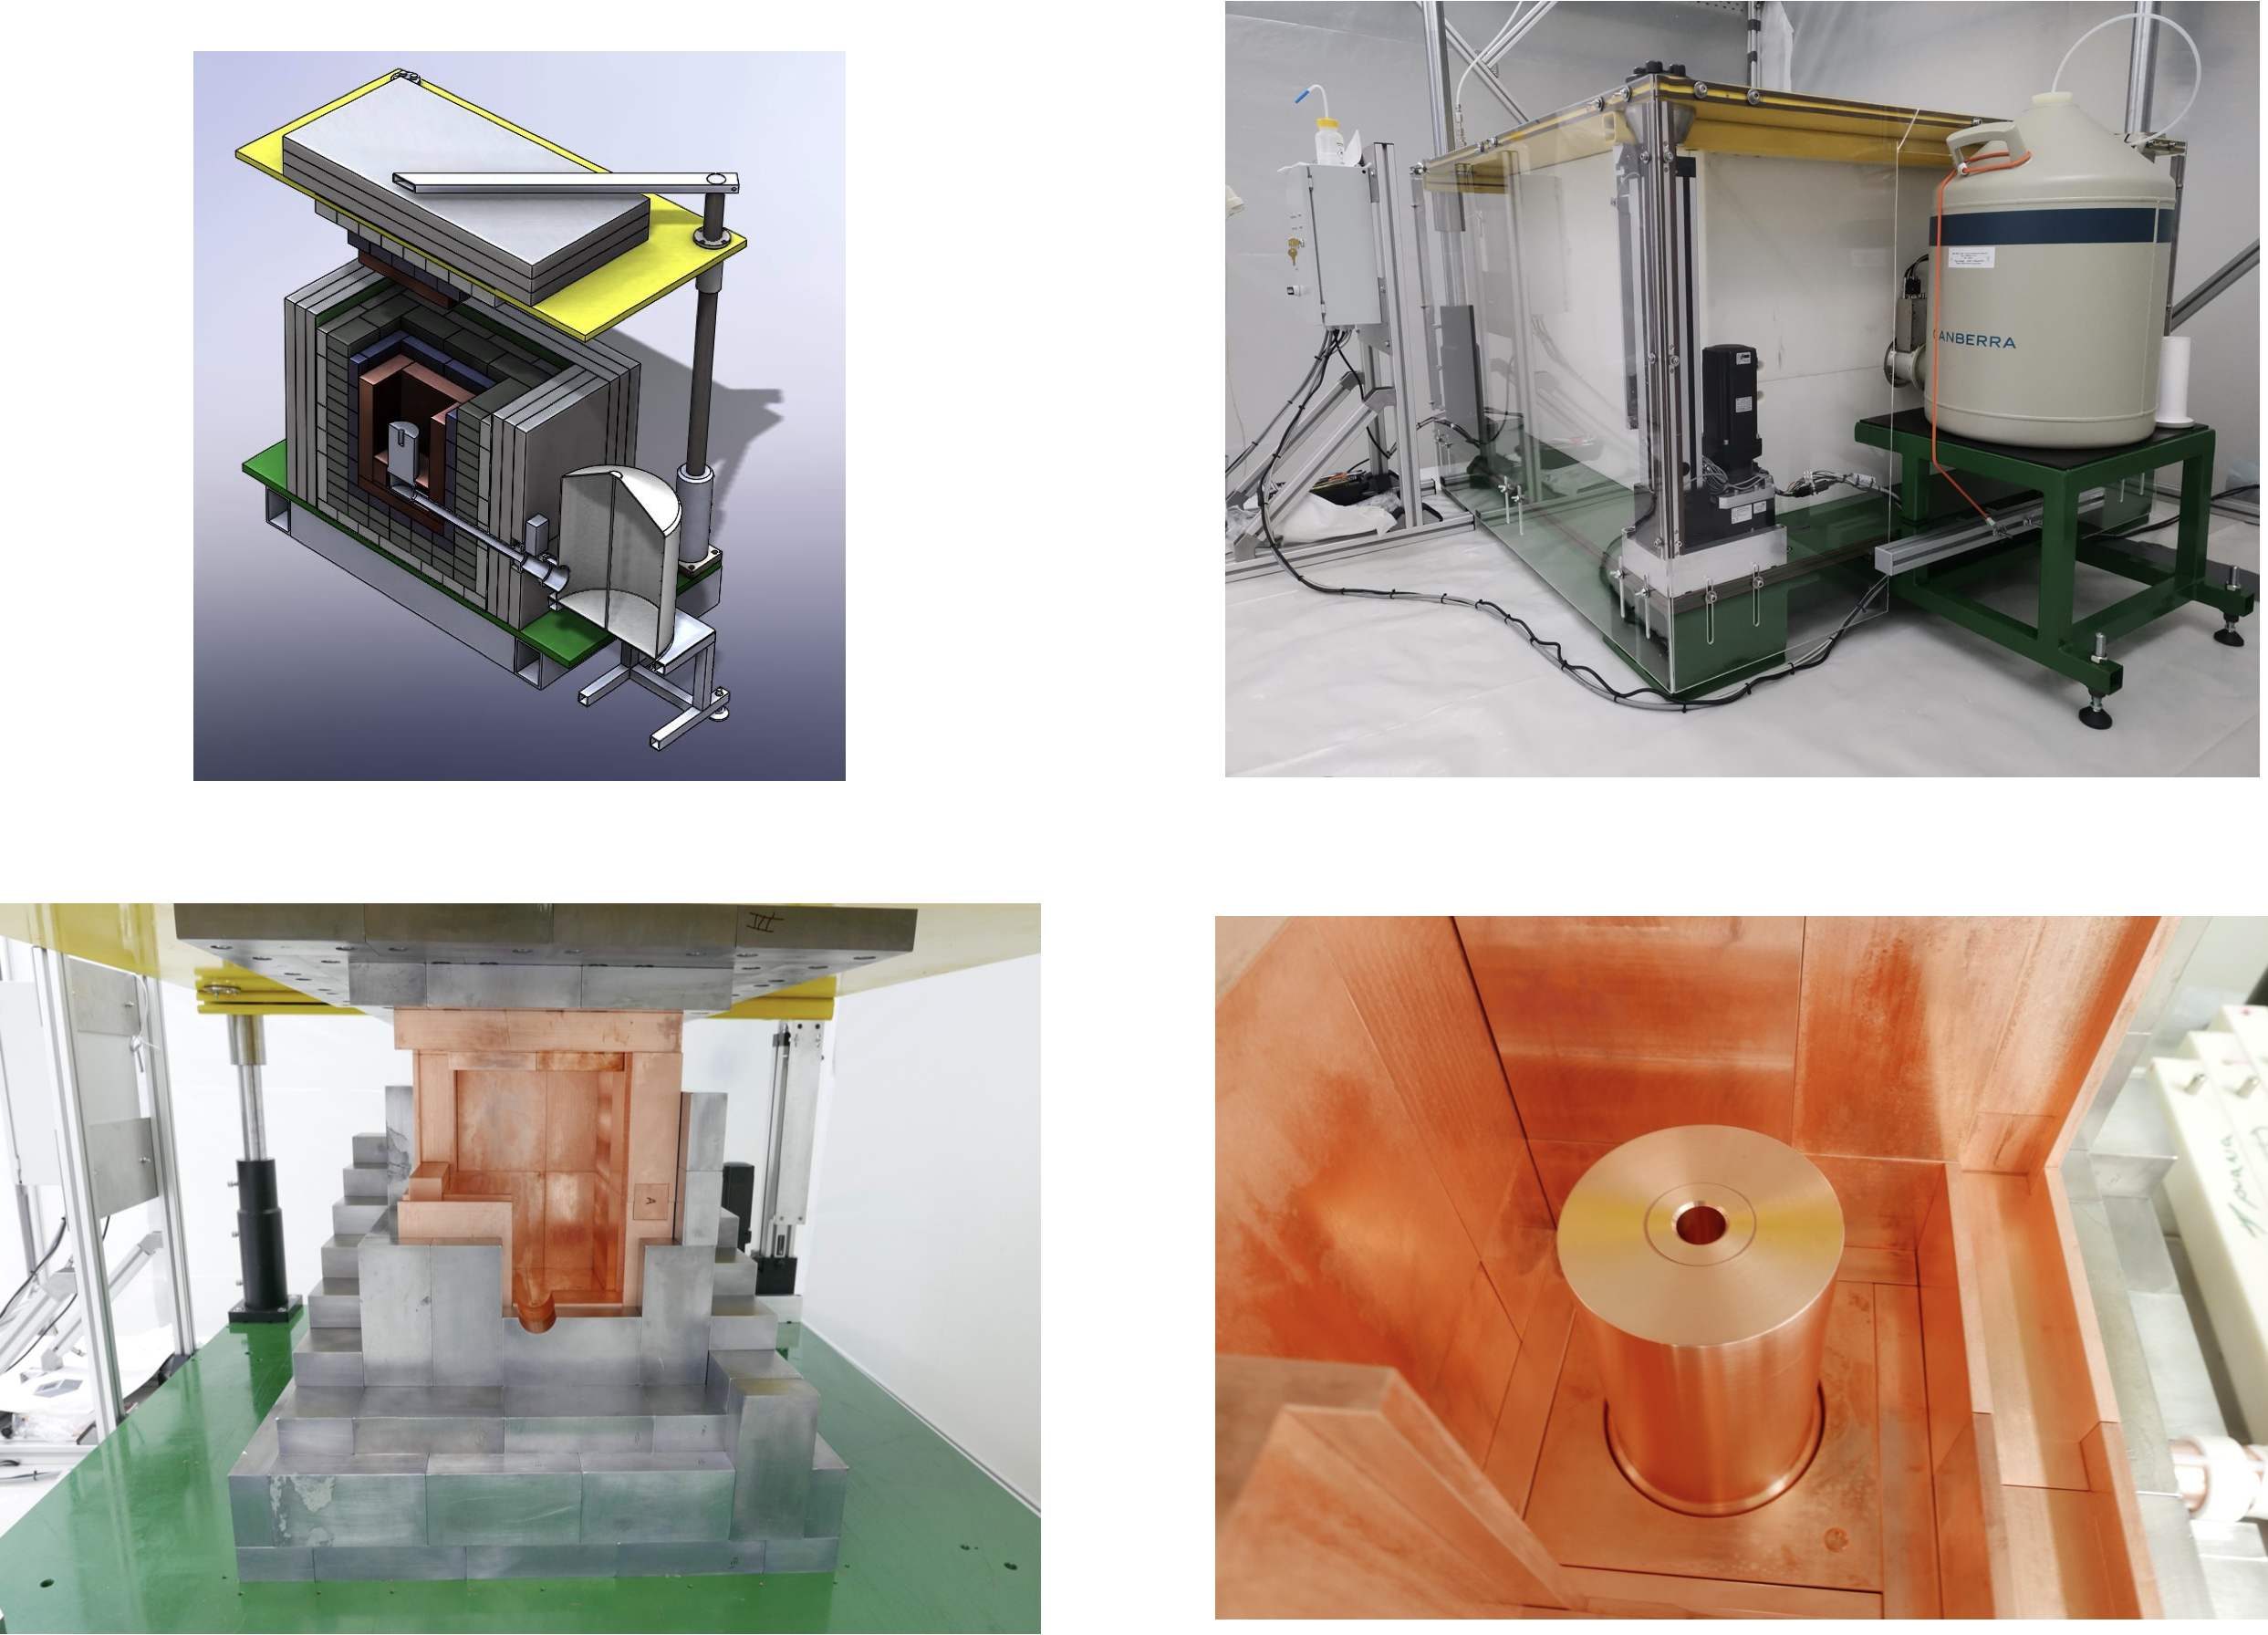
\includegraphics[scale=0.22]{anatomiaGe.png}

%Ambient background measured by a HPGe detector without and with (green) shield.
%
% \column{0.40\textwidth}
% 
%$\bullet~$ All \bbonu\  experiment must use materials with extremely low amounts of radioactive impurities. Selection, manufacturing, cleaning and installation of detector materials has to be conducted with extreme care in all \bbonu\  experiments, relying on radio-pure protocols at all times.
%
%\end{columns}
\end{frame}



\begin{frame}{Exercise 4}

$\bullet~$ Let us build a toy detector based on xenon. The vessel will be made of ultra-low radioactivity copper. The best such materials have activities in the chain of
${}^{238}$U of the order o 3 $\mu$Bq/kg. Assume that your pressure vessel is a cylinder with walls (and end-caps) 10 cm thick. Design the dimensions of the pressure vessel to contain one ton of xenon at 20 bar and one one of LXe. Then, compute the mass of your vessel and from that the total activity (in both cases). 

$\bullet~$ Refine your calculation computing only the activity that enters the active xenon volume. This means that you need to take into account geometrical and self-shielding effects. Write a small Monte Carlo to do the calculation or use analytical approximations.

$\bullet~$ Which activity do you get? What do you conclude from there?
\end{frame}

%\begin{frame}{Exercise 5}
%
%$\bullet~$ Assuming that your material is in equilibrium, all decays of ${}^{238}$U will lead to
%${}^{214}$Bi. About 1.5 \% of ${}^{214}$Bi decays will produce a gamma of energy 2.48 MeV, which is very close to \XE\ \qbb\ and thus becomes a very dangerous background. Assuming the activity in the steel in the exercise 4, you can compute now the total number of gammas of 2.48 MeV that cross the xenon volume. A fraction of those gammas will interact in the gas. You can compute that fraction using the NIST (\url{https://www.nist.gov/pml/x-ray-and-gamma-ray-data}) tables or Geant4. How many interactions do you get? What do you conclude?
%
%\end{frame}

\begin{frame}{Radioactive Earth}
\begin{columns}
\column{0.50\textwidth}
%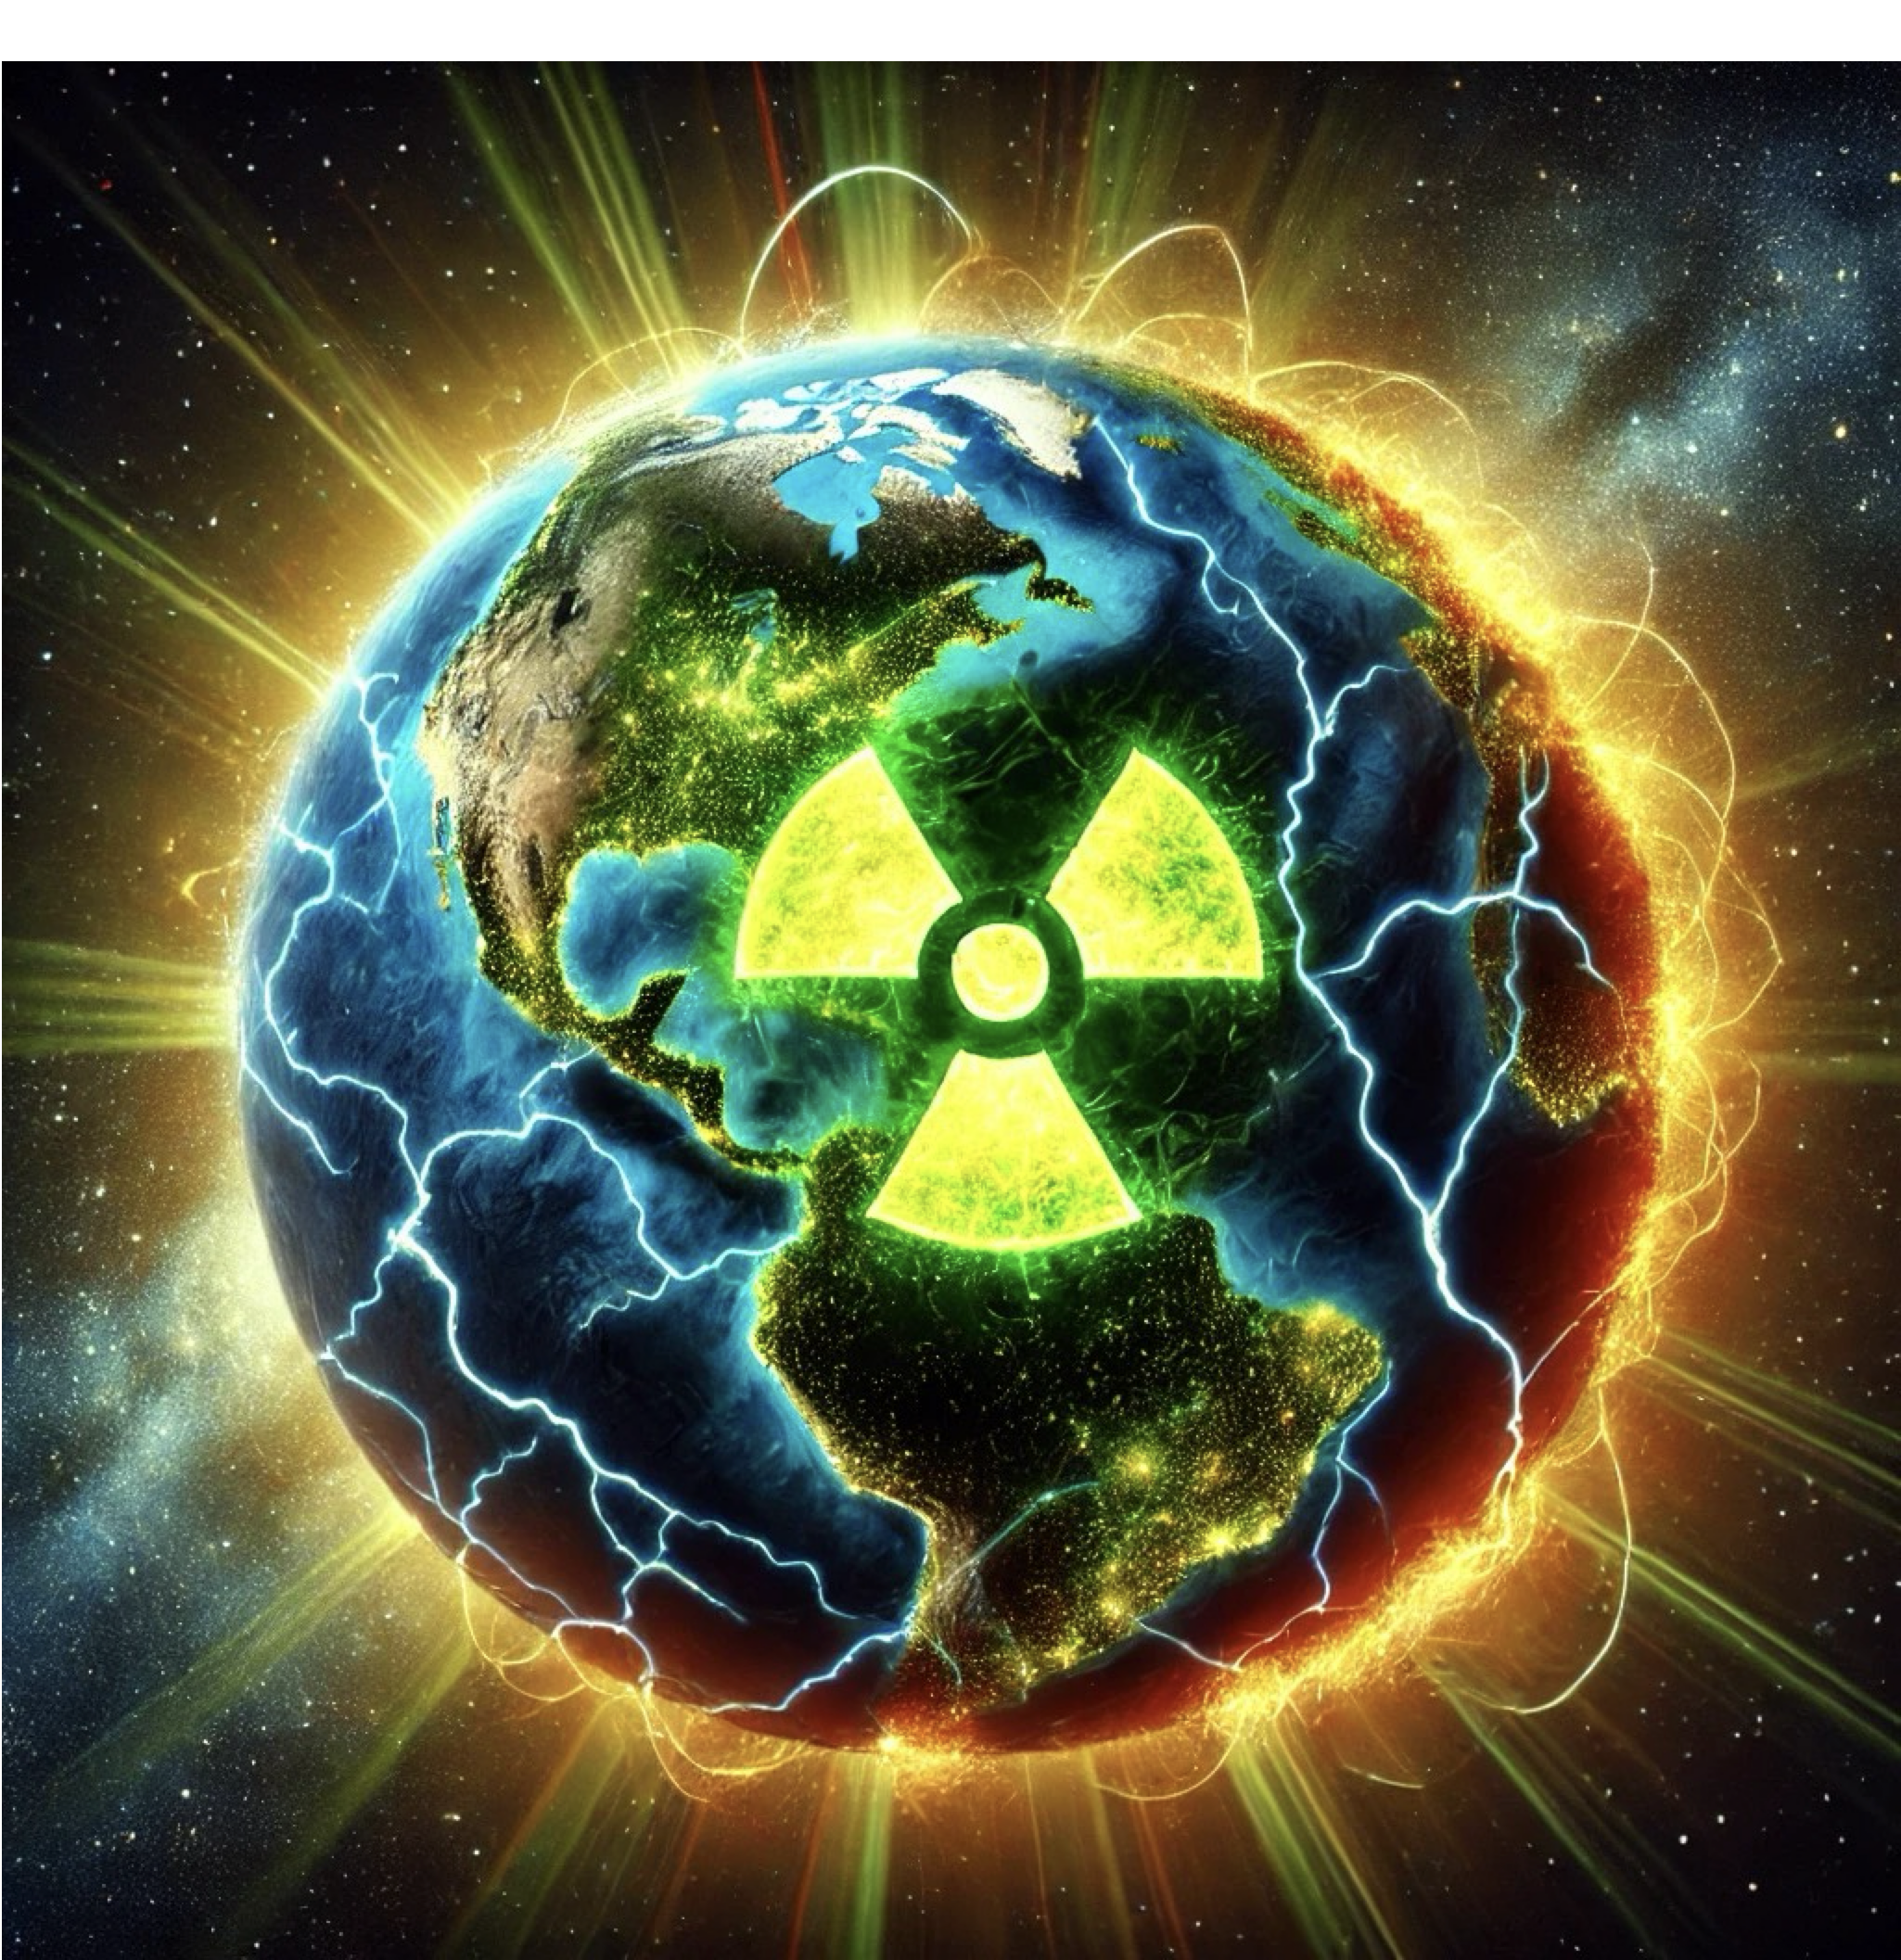
\includegraphics[scale=0.20]{radioactiveEarth.png}
\includegraphics[scale=0.40]{rchains.png}

 \column{0.50\textwidth}
$\bullet~$ Earth is a very radioactive planet. There is about 2-3 grams of U/Th per ton of rock. Everything, with the exception of ultra-pure metals tend to be more radioactive than \bbonu\ experiments can tolerate.   

$\bullet~$ The core of the business, then, is to combine sophisticated detection techniques with ultra-low radioactivity techniques. This, at the same time that one exploits suitable \bbonu\ isotopes to operate both as target and detector.   

\end{columns}
\end{frame}


\begin{frame}{Exercise 6}
\begin{columns}
\column{0.50\textwidth}
\includegraphics[scale=0.20]{snemo.png}

 \column{0.50\textwidth}
$\bullet~$ A priory one could design an experiment in which source and detector are not the same. In fact, the NEMO-3 detector measured \tonu\ for many isotopes using such an apparatus, in which the isotopes where introduced into the detector (tracker + calorimeter) as thin sheets of target material.    

$\bullet~$ The idea was then extended to the Super-Nemo detector, as in the figure. Each module of SN holds about 10 kg of isotope. 

$\bullet~$ {\bf Exercize 5}. Explain the advantages and disadvantages of the technique, in particular to reach a sensitivity of around $10^{27}$~y.   

\end{columns}
\end{frame}

\begin{frame}{A simple sensitivity formula (background free)}
$\bullet~$ Background-free experiment: consider an almost ideal experiment, capable to fully suppress backgrounds, at the cost of a selection efficiency $\epsilon$. If after running for a given exposure $M \cdot t$ no events are observed, we can establish a limit on \mbb\, to first approximation as:
\[
\mbb = \sqrt{\frac{W}{N_A}\cdot \frac{1}{\gonu\cdot\monu}\cdot \frac{1}{\epsilon\cdot M \cdot t}}
\]

$\bullet~$ Where $W$ is the molar mass, $N_A$ is the Avogadro number, \gonu\ is the phase space factor and \monu\ the NME for the isotope. 

$\bullet~$ {\bf Exercise 6}: Obtain limits for \XE\, \TE\, \GE\ and \MO. In each case assume
$M \cdot t = 1$~ton$\cdot$yr (do it also for $M \cdot t = 10$~ton$\cdot$yr) , and $\epsilon =1$ (truly ideal detector). 
\end{frame}


%%%
\begin{frame}{A simple sensitivity formula (background)}
$\bullet~$ Background experiment: consider an experiment in which a number of events $b~$ are observed (and sufficiently large to be in gaussian regime), we can establish a limit on \mbb\, to first approximation as:
\[
\mbb = \sqrt{\frac{W}{N_A}\cdot \frac{b^{1/2}}{\gonu\cdot\monu}\cdot \frac{1}{\epsilon\cdot M \cdot t}}
\]

$\bullet~$ Write now, $b = c \cdot M \cdot t \cdot \Delta E$, where c is rate (assumed constant) of events in the ROI, defined by the resolution $\Delta E$. Then: 

\[
\mbb = (\frac{\alpha^2 \cdot \beta}{\epsilon^2})^{1/4}
\]

where
\[
\alpha = (\frac{W/N_A}{\gonu\cdot\monu}), \, \, \, \beta = \frac{c\cdot \Delta E}{M\cdot t}
\]
\end{frame}

%%%%

\begin{frame}{The $\alpha$ term}
$\bullet~$ The $\alpha$ term depends on the physical properties of the isotope.

 $\bullet~$ Notice that it enters the equation with a square.
 
 $\bullet~$ Since $N_A$ is constant, $\alpha \propto W/(\gonu\monu)$. Notice that one would like to select isotopes as light as possible (small $W$) with phase space and NME as large as possible. 
 
 $\bullet~$ {\bf Exercise 7}: Compute $\alpha$ for \XE\, \TE\, \GE\ and \MO. 
 \end{frame}
 
 %%%%
 
 \begin{frame}{The $\beta$ term and $\epsilon$}
$\bullet~$ The $\beta$ term depends on the experimental technique. Notice that the product of background rate and energy resolution compensates exactly the exposure. 

 $\bullet~$ On the other hand, notice that the selection efficiency enters the formula with a square, motivating experimental techniques with $\epsilon \sim 1$. 
 
 $\bullet~$ Not all parameters can be optimised at the same time. Notice that a possible approach is to go for very large masses (KamLAND-Zen, SNO+), while another is to bet on extremely good energy resolution (GERDA/LEGEND). Other experiments may try a combination of the three parameters (NEXT, NEXO, CUPID). One can even, conceivably try an approach in which $c \sim 0$ (NEXT-BOLD). 
 
 \end{frame}
 
 %%%%%%%%%%
 
 \begin{frame}{The saddest woe of the business}
 
 \begin{columns}
\column{0.50\textwidth}
\begin{figure}
\includegraphics[scale=0.28]{ gesensi.png}
\caption{3. Sensitivity of \GE\ experiment as a function of the background rate}
\end{figure}

 \column{0.50\textwidth}
$\bullet~$ Notice that the sensitivity of the experiment only improves with (1/4)th power, that is extremely slowly. In other words, for a given target on sensitivity, experiments must attempt to reach a ``background free" regime, or pay dearly in exposure as clearly seen in the graphics.

$\bullet~$ A background free Ge experiment, ``Legend-like", would reach a sensitivity of $\sim 10^{28}$~yr with a exposure of 2 ton$\cdot$year. With a background of only 1 count per ton$\cdot$ year in the ROI, the exposure becomes... 100 years!!! That is, impossible. 
\end{columns}
\end{frame}

\begin{frame}{Exercise 8}
$\bullet~$ Reproduce the plot in the previous transparency for the four isotopes that we are considering (assume $\epsilon =1$ for all of them). 
\end{frame}

\begin{frame}{How to build the next generation of \bbonu\ experiments}
$\bullet~$ Figure 3 disclosures the best kept secrets of the business (do not tell funding agencies or prospective graduate students).
 
 $\bullet~$ {\bf The secret}: Reaching a sensitivity of $\tonu \sim 10^{27}$ requires an exposure of several ton$\cdot$year, with a tolerance of about 1 background event per year in the ROI.
 
 $\bullet~$ {\bf The Uber-secret}: Reaching a sensitivity of $\tonu \sim 10^{28}$ requires an exposure of several tens of ton$\cdot$year, with a tolerance of about 0.1 background event per year in the ROI.
 
 $\bullet~$ {\bf Old Spanish Wisdom}: Impossible things are those that require a miracle. Truly impossible things are those that cannot be done even by miracle. And then, there are \bbonu\ searches.
 
 \end{frame}
 
 \begin{frame}{Exercise 9}
$\bullet~$ As we have discussed, our uber-experiment to search for \bbonu\ can tolerate about 1 (0.1) events of background per year in the ROI. Discuss how to evaluate the error on that quantity. What should be the order of magnitude of the error in each case?
\end{frame}
 

\end{document}